% ============================================================================
% AOGS pipeline flowchart — how the discrete-layer study computes, WITH the
% governing equations at each step and the actual K_d used in each branch.
% Teal = new in this study; gray = the established certified baseline pipeline.
% Build:  /Library/TeX/texbin/pdflatex aogs_pipeline_flowchart.tex
% PNG:    python3 -c "import fitz; fitz.open('aogs_pipeline_flowchart.pdf')[0].get_pixmap(dpi=300).save('aogs_pipeline_flowchart.png')"
% ============================================================================
\documentclass[tikz, border=8pt]{standalone}
\usepackage[T1]{fontenc}
\usepackage{newtxtext,newtxmath}
\usetikzlibrary{positioning, arrows.meta, calc}

% house palette (lunar.plotting.style)
\definecolor{teal}{HTML}{2A6478}
\definecolor{char}{HTML}{2A2520}
\definecolor{gridc}{HTML}{E8E5E0}
\definecolor{dim}{HTML}{8A857E}
\definecolor{coral}{HTML}{B85B3A}

\begin{document}
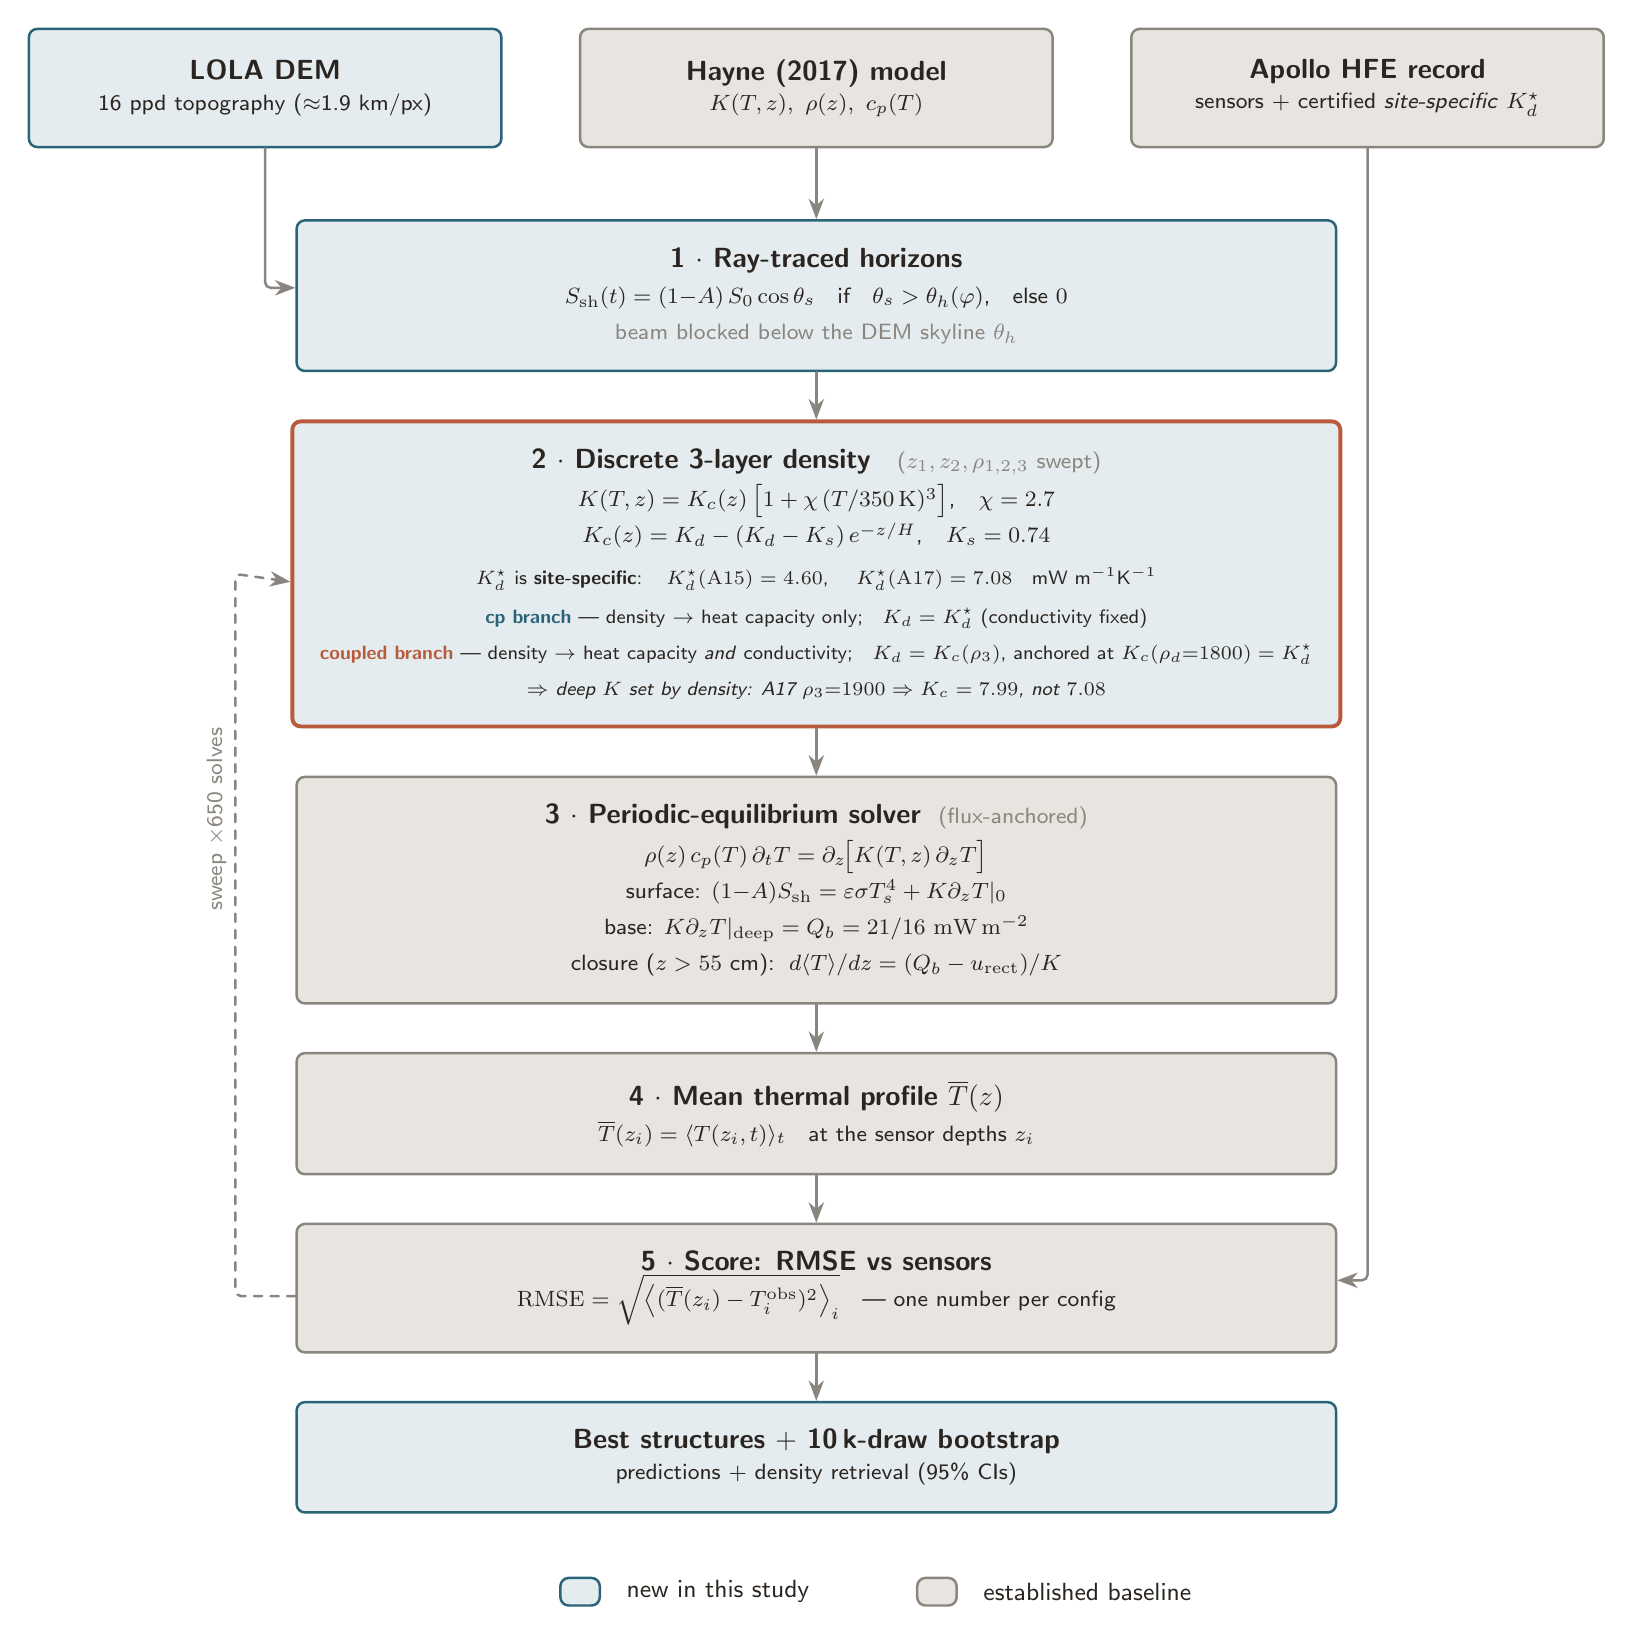
\begin{tikzpicture}[
  font=\sffamily,
  new/.style={draw=teal, line width=0.9pt, fill=teal!12, rounded corners=3pt,
              align=center, text=char, minimum width=132mm, inner sep=3.5mm},
  old/.style={draw=dim, line width=0.9pt, fill=gridc, rounded corners=3pt,
              align=center, text=char, minimum width=132mm, inner sep=3.5mm},
  key/.style={draw=coral, line width=1.4pt, fill=teal!12, rounded corners=3pt,
              align=center, text=char, minimum width=132mm, inner sep=3.5mm},
  inp/.style={draw, line width=0.9pt, rounded corners=3pt, align=center,
              text=char, minimum width=60mm, minimum height=15mm},
  lbl/.style={font=\sffamily\small, text=char},
  sub/.style={font=\sffamily\footnotesize, text=dim},
  arr/.style={-{Stealth[length=2.6mm]}, line width=0.9pt, draw=dim,
              rounded corners=2pt, line cap=round},
  eq/.style={font=\footnotesize},          % equations
  eqs/.style={font=\scriptsize},           % sub-equations / notes
]

% ── inputs row ───────────────────────────────────────────────────────────────
\node[inp, draw=teal, fill=teal!12] (dem) at (-7.0, 0)
    {\textbf{LOLA DEM}\\[-1pt]{\footnotesize 16 ppd topography ($\approx$1.9 km/px)}};
\node[inp, draw=dim, fill=gridc] (hay) at (0, 0)
    {\textbf{Hayne (2017) model}\\[-1pt]{\footnotesize $K(T,z),\ \rho(z),\ c_p(T)$}};
\node[inp, draw=dim, fill=gridc] (hfe) at (7.0, 0)
    {\textbf{Apollo HFE record}\\[-1pt]{\footnotesize sensors $+$ certified
     \emph{site-specific} $K_d^{\star}$}};

% ── spine ────────────────────────────────────────────────────────────────────
\node[new, below=9mm of hay] (s1)
    {\textbf{1 $\cdot$ Ray-traced horizons}\\[1pt]
     {\footnotesize $S_{\rm sh}(t)=(1{-}A)\,S_0\cos\theta_s$ \; if \;
      $\theta_s>\theta_h(\varphi)$, \; else $0$}\\[1pt]
     {\footnotesize\color{dim} beam blocked below the DEM skyline $\theta_h$}};

\node[key, below=6mm of s1] (s2)
    {\textbf{2 $\cdot$ Discrete 3-layer density}
     \; {\footnotesize\color{dim}($z_1,z_2,\rho_{1,2,3}$ swept)}\\[2pt]
     {\footnotesize $K(T,z)=K_c(z)\,\big[1+\chi\,(T/350\,\mathrm{K})^{3}\big]$,\quad
      $\chi=2.7$}\\[1pt]
     {\footnotesize $K_c(z)=K_d-(K_d-K_s)\,e^{-z/H}$,\quad $K_s=0.74$}\\[3pt]
     {\scriptsize $K_d^{\star}$ is \textbf{site-specific}: \;
      $K_d^{\star}(\mathrm{A15})=4.60$, \quad $K_d^{\star}(\mathrm{A17})=7.08$
      \; mW m$^{-1}$K$^{-1}$}\\[2pt]
     {\scriptsize\textbf{\color{teal}cp branch} --- density $\to$ heat capacity
      only; \; $K_d=K_d^{\star}$ (conductivity fixed)}\\[1pt]
     {\scriptsize\textbf{\color{coral}coupled branch} --- density $\to$ heat
      capacity \emph{and} conductivity; \; $K_d=K_c(\rho_3)$, anchored at
      $K_c(\rho_d{=}1800)=K_d^{\star}$}\\[1pt]
     {\scriptsize\emph{$\Rightarrow$ deep $K$ set by density: A17 $\rho_3{=}1900
      \Rightarrow K_c=7.99$, not $7.08$}}};

\node[old, below=6mm of s2] (s3)
    {\textbf{3 $\cdot$ Periodic-equilibrium solver}
     \;{\footnotesize\color{dim}(flux-anchored)}\\[2pt]
     {\footnotesize $\rho(z)\,c_p(T)\,\partial_t T=\partial_z\!\big[K(T,z)\,\partial_z T\big]$}\\[1pt]
     {\footnotesize surface: $(1{-}A)S_{\rm sh}=\varepsilon\sigma T_s^{4}+K\partial_z T|_0$}\\[1pt]
     {\footnotesize base: $K\partial_z T|_{\rm deep}=Q_b=21/16\ \mathrm{mW\,m^{-2}}$}\\[1pt]
     {\footnotesize closure ($z>55$ cm): $\,d\langle T\rangle/dz=(Q_b-u_{\rm rect})/K$}};

\node[old, below=6mm of s3] (s4)
    {\textbf{4 $\cdot$ Mean thermal profile $\overline{T}(z)$}\\[1pt]
     {\footnotesize $\overline{T}(z_i)=\langle T(z_i,t)\rangle_t$ \; at the sensor depths $z_i$}};

\node[old, below=6mm of s4] (s5)
    {\textbf{5 $\cdot$ Score: RMSE vs sensors}\\[1pt]
     {\footnotesize $\mathrm{RMSE}=\sqrt{\big\langle(\overline{T}(z_i)-T_i^{\rm obs})^{2}\big\rangle_i}$
      \; --- one number per config}};

\node[new, below=6mm of s5] (out)
    {\textbf{Best structures $+$ 10\,k-draw bootstrap}\\[-1pt]
     {\footnotesize predictions $+$ density retrieval (95\% CIs)}};

% ── connectors ───────────────────────────────────────────────────────────────
\draw[arr] (hay.south) -- (s1.north);
\draw[arr] (dem.south) |- ($(s1.west)+(0,0.10)$);
\draw[arr] (hfe.south) |- ($(s5.east)+(0,0.10)$);
\draw[arr] (s1.south) -- (s2.north);
\draw[arr] (s2.south) -- (s3.north);
\draw[arr] (s3.south) -- (s4.north);
\draw[arr] (s4.south) -- (s5.north);
\draw[arr] (s5.south) -- (out.north);

% sweep loop (left side, dashed)
\draw[arr, dashed] ($(s5.west)+(0,-0.10)$) -| ($(s2.west)+(-0.7,0)$)
                   -- ($(s2.west)+(0,-0.10)$);
\node[sub, rotate=90] at ($(s3.west)+(-1.0,0.9)$) {sweep $\times$650 solves};

% ── legend ───────────────────────────────────────────────────────────────────
\node[new, minimum width=5mm, minimum height=3.5mm, below=8mm of out,
      xshift=-30mm, inner sep=0pt] (lg1) {};
\node[lbl, right=2mm of lg1] {new in this study};
\node[old, minimum width=5mm, minimum height=3.5mm, right=10mm of lg1,
      xshift=30mm, inner sep=0pt] (lg2) {};
\node[lbl, right=2mm of lg2] {established baseline};

\end{tikzpicture}
\end{document}
